\documentclass[conference]{IEEEtran}
\IEEEoverridecommandlockouts
\usepackage{cite}
\usepackage{amsmath,amssymb,amsfonts}
\usepackage{algorithmic}
\usepackage{graphicx}
\usepackage{textcomp}
\usepackage{xcolor}
\usepackage{booktabs}
\usepackage{array}
\usepackage{url}
\usepackage{tikz}
\usetikzlibrary{arrows.meta,positioning,calc,fit}
\usepackage{pgfplots}
\pgfplotsset{compat=1.16,
  every axis/.append style={font=\scriptsize, tick label style={font=\scriptsize}, label style={font=\scriptsize}, legend style={font=\tiny}}}
\def\BibTeX{{\rm B\kern-.05em{\sc i\kern-.025em b}\kern-.08em
    T\kern-.1667em\lower.7ex\hbox{E}\kern-.125emX}}


\begin{document}

\title{Parameter-Efficient Adaptation of Multilingual Transformers for Telugu Abusive Comment Detection}

\author{\IEEEauthorblockN{1\textsuperscript{st} Given Name Surname}
\IEEEauthorblockA{\textit{dept. name of organization} \\
\textit{name of organization}\\
City, Country \\
email address or ORCID}
\and
\IEEEauthorblockN{2\textsuperscript{nd} Given Name Surname}
\IEEEauthorblockA{\textit{dept. name of organization} \\
\textit{name of organization}\\
City, Country \\
email address or ORCID}
\and
\IEEEauthorblockN{3\textsuperscript{rd} Given Name Surname}
\IEEEauthorblockA{\textit{dept. name of organization} \\
\textit{name of organization}\\
City, Country \\
email address or ORCID}
}

\maketitle

\begin{abstract}
Automatic detection of abusive comments in low-resource Indian languages is constrained by computational budgets, by the absence of statistically controlled comparisons between adaptation methods, and by users who disguise abusive words. This paper presents a controlled study of parameter-efficient fine-tuning for Telugu abusive comment detection on the Telugu portion of the MACD corpus. Full fine-tuning, LoRA, DoRA and AdaLoRA are compared on XLM-RoBERTa, MuRIL, multilingual BERT and IndicBERT v2 with three random seeds, against a TF-IDF and linear SVM baseline. Configurations are selected on validation macro-F1 only, and differences are assessed with paired bootstrap intervals and McNemar tests on identical test comments. LoRA on the attention query and value matrices of XLM-RoBERTa reaches 0.9035 test macro-F1 against 0.9057 for full fine-tuning, while training 0.32\% of the parameters and requiring about one third of the GPU memory; the difference is not statistically detectable. DoRA yields no gain and AdaLoRA is significantly worse. The TF-IDF baseline reaches 0.9029 and is statistically indistinguishable from the adapted transformers. A rule-based input guard that reverses character-level disguises raises mean accuracy under twenty attacks from approximately 0.71 to 0.86 for every classifier evaluated. Advertisement-like template posts account for about 15\% of abusive comments and inflate all scores by approximately 0.8 points without altering the ranking of systems. A calibrated allow, review and block pipeline built on a 3.4~MB adapter is described, together with the cases in which the expected benefits of newer adaptation methods did not materialize.
\end{abstract}

\begin{IEEEkeywords}
abusive language detection, Telugu, low-resource languages, parameter-efficient fine-tuning, LoRA, DoRA, AdaLoRA, XLM-RoBERTa, calibration
\end{IEEEkeywords}

\section{Introduction}
Abusive comments are a persistent problem on social platforms, and moderation for Indian languages is harder than for English because labeled data, pretrained models and tooling are less mature. Telugu is spoken by more than 80 million people, yet it has far fewer public benchmarks than English. Early work framed the task as classification of short texts with lexical features \cite{waseem2016,davidson2017}, and surveys document the shift towards neural models \cite{schmidt2017}. Pretrained transformer encoders \cite{vaswani2017,devlin2019bert} now provide strong accuracy, but fully fine-tuning a 278-million-parameter model for every language, task or domain is costly in memory, storage and time. Parameter-efficient fine-tuning (PEFT) keeps the pretrained weights frozen and trains small additional modules \cite{houlsby2019,hu2022lora}, which makes per-task adapters of a few megabytes practical.

The closest prior work applies LoRA to hate speech detection in another low-resource language \cite{kaunang2026indo}, but without a full fine-tuning reference, competing adaptation methods, a classical baseline, seed variance or significance testing, and without examining robustness or deployment. Whether parameter-efficient adaptation is a sound choice for Telugu, and at what cost, therefore remains open. This study addresses that question and makes the following contributions.
\begin{enumerate}
\item A controlled comparison of full fine-tuning, LoRA, DoRA and AdaLoRA on four multilingual encoders on the Telugu part of MACD \cite{gupta2022macd}, with three seeds, validation-only selection, and recorded trainable parameters, memory, time and adapter size.
\item Paired significance tests (bootstrap and McNemar) on identical test comments, and a replication of the published LoRA recipe \cite{kaunang2026indo} alongside the tuned configuration, which raises mean test macro-F1 from 0.8985 to 0.9035, although the paired difference is not statistically significant.
\item A classical TF-IDF baseline and an input-guard ablation showing that, on this corpus, neither the transformer nor its adaptation method is the main source of accuracy or robustness.
\item A deployable pipeline with temperature scaling, review thresholds and INT8 export, including an audit that found a per-tensor INT8 export unusable.
\item An error and data analysis showing that 42\% of the selected model's errors are shared by all five strong systems and that about 15\% of abusive comments are advertisement-like templates.
\end{enumerate}

The remainder of the paper is organized as follows. Section~\ref{sec:related} reviews related work and identifies the research gaps. Section~\ref{sec:method} describes the data, models, training protocol and deployment pipeline. Section~\ref{sec:results} reports and discusses the results, and Section~\ref{sec:concl} concludes.

\section{Related Work}
\label{sec:related}
\subsection{Abusive comment detection and MACD}
MACD is a multilingual corpus of about 150,000 user comments from a social platform covering five Indic languages, released with the AbuseXLMR model \cite{gupta2022macd}. The Telugu portion, which comprises roughly 24,000 training, 3,000 validation and 3,000 test comments with a binary label (abusive or not), is used throughout this study.

\subsection{Multilingual encoders}
The study evaluates four pretrained encoders. XLM-RoBERTa (XLM-R) is trained on CommonCrawl text in 100 languages \cite{conneau2020xlmr}. MuRIL is a BERT model pretrained on Indian languages, including transliterated text \cite{khanuja2021muril}. Multilingual BERT (mBERT) is the original BERT recipe trained on Wikipedia in 104 languages \cite{devlin2019bert}. IndicBERT v2 is trained on the IndicCorp v2 corpus of 24 Indic languages \cite{doddapaneni2023indicbert}. The original IndicBERT checkpoint was not accessible, so IndicBERT v2 is used in its place.

\subsection{Parameter-efficient fine-tuning}
Adapter layers insert small trainable modules between frozen layers \cite{houlsby2019}; prefix and prompt tuning learn continuous vectors prepended to the input \cite{li2021prefix,lester2021prompt}. The success of such methods is often explained by the low intrinsic dimensionality of fine-tuning \cite{aghajanyan2021intrinsic}. LoRA freezes a pretrained weight matrix $W_0$ and learns a low-rank update, so that
\begin{equation}
W = W_0 + \frac{\alpha}{r}BA,\qquad B\in\mathbb{R}^{d\times r},\; A\in\mathbb{R}^{r\times k},\; r\ll\min(d,k),
\label{eq:lora}
\end{equation}
as in \cite{hu2022lora} and Fig.~\ref{fig:lora}. DoRA splits the weight into a magnitude vector and a direction and applies the low-rank update to the direction \cite{liu2024dora}. AdaLoRA parameterizes the update in singular-value form and prunes ranks by importance under a global budget \cite{zhang2023adalora}. QLoRA and $(IA)^3$ are further PEFT variants \cite{dettmers2023qlora,liu2022ia3}. All adapter methods use the PEFT library implementations \cite{mangrulkar2022peft}.

\begin{figure}[t]
\centering
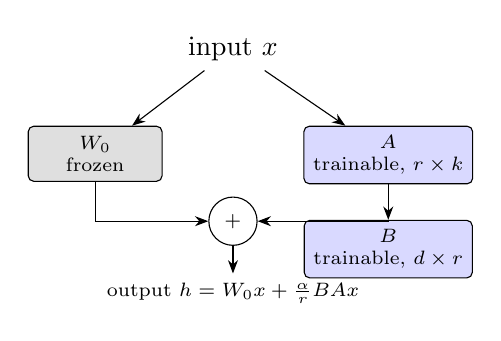
\begin{tikzpicture}[>=Stealth, block/.style={draw, rounded corners=2pt, font=\scriptsize, align=center, minimum height=0.7cm, minimum width=1.7cm}]
\node (x) {input $x$};
\node[block, fill=gray!25, below left=0.7cm and 0.2cm of x] (w) {$W_0$\\frozen};
\node[block, fill=blue!15, below right=0.7cm and 0.2cm of x] (a) {$A$\\trainable, $r\times k$};
\node[block, fill=blue!15, below=0.45cm of a] (b) {$B$\\trainable, $d\times r$};
\node[draw, circle, font=\scriptsize, below=1.6cm of x] (p) {$+$};
\node[font=\scriptsize, below=0.35cm of p] (h) {output $h=W_0x+\frac{\alpha}{r}BAx$};
\draw[->] (x) -- (w);
\draw[->] (x) -- (a);
\draw[->] (a) -- (b);
\draw[->] (w) |- (p);
\draw[->] (b) |- (p);
\draw[->] (p) -- (h);
\end{tikzpicture}
\caption{LoRA keeps the pretrained matrix $W_0$ frozen and trains only the two thin matrices $A$ and $B$; their product is added to the output.}
\label{fig:lora}
\end{figure}

\subsection{Evasion of abuse detectors}
Detectors are known to be brittle to small edits such as inserted characters, spacing and typos \cite{hosseini2017,grondahl2018}. This motivates the rule-based input guard and the attack-based evaluation in Section~\ref{sec:results}.

\subsection{Research gaps in existing solutions}
A recent study applied LoRA to IndoBERT for Indonesian hate speech across several platforms \cite{kaunang2026indo}. Its recipe, adapting only the query and value projections at a small rank, is attractive for Telugu, but the study leaves several questions open that the present work addresses (Table~\ref{tab:gaps}). The reference reports no comparison against full fine-tuning, so the accuracy cost of adaptation is unknown. Newer variants (DoRA, AdaLoRA) and alternative backbones are not evaluated. No classical baseline is given, so the benefit of a transformer is unquantified. Results come from a single run without variance across seeds or significance tests. Finally, robustness to deliberate disguise and deployment concerns (calibration, quantization) are not examined. The MACD benchmark \cite{gupta2022macd} supplies Telugu data and a fully fine-tuned baseline, but it does not study adapter methods, and work on evasion \cite{hosseini2017,grondahl2018} has not been connected to Indic-language PEFT classifiers.

\begin{table}[t]
\caption{Gaps in existing solutions and the corresponding contribution of this work.}
\label{tab:gaps}
\centering
\footnotesize
\begin{tabular}{>{\raggedright\arraybackslash}p{2.5cm}>{\raggedright\arraybackslash}p{2.4cm}>{\raggedright\arraybackslash}p{2.7cm}}
\toprule
Gap & Existing work \cite{kaunang2026indo} & This work \\
\midrule
Full fine-tuning reference & Absent & Four backbones, three seeds \\
Newer PEFT methods & LoRA only & LoRA, DoRA, AdaLoRA \\
Classical baseline & Absent & TF-IDF + linear SVM \\
Variance and significance & Single run & Bootstrap, McNemar, seeds \\
Selection protocol & Not stated & Validation-only tie-set rule \\
Robustness to disguise & Not examined & 20 attacks, input guard \\
Deployment & Not examined & Calibration, INT8 audit \\
Data artifacts & Not examined & Template-post analysis \\
\bottomrule
\end{tabular}
\end{table}

\section{Methodology}
\label{sec:method}
\subsection{Data and preprocessing}
Rows with missing fields and exact duplicates within each split were removed, and comments of the validation and test splits that also occur verbatim in the training split were then dropped (2 and 3 comments, respectively). Table~\ref{tab:data} gives the resulting sizes. The released files use 0 for abusive and 1 for non-abusive; this was verified against the upstream release and remapped to 1 = abusive throughout. Text is Unicode-normalized (NFC), URLs and mentions are masked and whitespace is collapsed; punctuation, emoji and repeated characters are kept, because they can carry abuse signals. The lowercasing and symbol stripping used for Indonesian text in \cite{kaunang2026indo} is not applied.

\begin{table}[t]
\caption{Telugu MACD splits used in this study after duplicate removal.}
\label{tab:data}
\centering
\footnotesize
\begin{tabular}{lrrrr}
\toprule
Split & Comments & Abusive & Non-abusive & Mean words \\
\midrule
Train & 23,980 & 12,401 & 11,579 & 12.8 \\
Validation & 2,998 & 1,616 & 1,382 & 13.2 \\
Test & 2,997 & 1,561 & 1,436 & 12.7 \\
\bottomrule
\end{tabular}
\end{table}

\subsection{Models and training}
Each encoder serves as a sequence classifier with a binary head. For PEFT, the base model is frozen, adapters are placed on the attention \texttt{query} and \texttt{value} matrices, and the classification head is trained and saved. Table~\ref{tab:hp} lists the settings; all runs use AdamW \cite{loshchilov2019adamw} with weight decay 0.01, a cosine schedule with 10\% warmup and FP16. Rank $\{4,8,16,32\}$, alpha $\{16,32,64\}$ and learning rate $\{10^{-4},2\times10^{-4},5\times10^{-4}\}$ were searched on MuRIL with one seed, and the selected setting was reused for the other backbones; DoRA and AdaLoRA were therefore not tuned separately. The experiments also reproduce the published recipe of \cite{kaunang2026indo} and a $r=16$, $\alpha=32$ starting configuration unchanged on XLM-R. Every compared configuration uses seeds 42, 123 and 2024. All experiments ran on a single 8~GB RTX 4060 Ti with PyTorch 2.6, Transformers \cite{wolf2020transformers} 4.57 and PEFT 0.21.

\begin{table}[t]
\caption{Training settings. ``Published'' is the recipe of \cite{kaunang2026indo} applied unchanged.}
\label{tab:hp}
\centering
\footnotesize
\setlength{\tabcolsep}{3.5pt}
\begin{tabular}{lccc}
\toprule
Setting & This work (PEFT) & Full FT & Published \\
\midrule
Rank $r$ / alpha $\alpha$ & 8 / 64 & -- & 4 / 32 \\
LoRA dropout & 0.05 & -- & 0.1 \\
Target modules & query, value & all & query, value \\
Learning rate & $2\times10^{-4}$ & $2\times10^{-5}$ & $2\times10^{-4}$ \\
Batch size & 16 & 16 & 8 \\
Max length (tokens) & 96 & 96 & 128 \\
Epochs (maximum) & 10 & 5 & 5 \\
Early stopping & \multicolumn{3}{c}{patience 3 on validation macro-F1} \\
\bottomrule
\end{tabular}
\end{table}

\subsection{Classical baseline}
The baseline uses TF-IDF features from character 2--5-grams within word boundaries and word 1--2-grams, with a linear SVM \cite{cortes1995svm} implemented in scikit-learn \cite{pedregosa2011sklearn}. The regularization constant was chosen from $\{0.1,0.3,1,3,10\}$ on validation macro-F1 (the selected value is 0.3).

\subsection{Metrics}
Let TP, FP, FN and TN be the counts of true and false positives and negatives for the abusive class. Then
\begin{align}
P &= \frac{TP}{TP+FP}, \qquad R = \frac{TP}{TP+FN}, \qquad F_1 = \frac{2PR}{P+R},\\
\text{macro-}F_1 &= \tfrac{1}{2}\left(F_1^{\,\text{abusive}} + F_1^{\,\text{non-abusive}}\right),\\
\text{ECE} &= \sum_{b=1}^{B}\frac{|S_b|}{n}\,\bigl|\,\mathrm{acc}(S_b)-\mathrm{conf}(S_b)\,\bigr|,
\end{align}
where $S_b$ are confidence bins \cite{guo2017calibration}. Macro-F1 weights both classes equally \cite{sokolova2009}. Accuracy, weighted-F1 and the confusion matrix are also reported.

\subsection{Selection and statistical testing}
Model selection relies on validation scores only (Fig.~\ref{alg:select}): configurations with three seeds were ranked by mean validation macro-F1, all configurations within one standard deviation of the best form a tie set, and the member with the fewest trainable parameters is selected. The test set is read once per run, for reporting only. The selected model is compared with each alternative on the same 2,997 test comments using a paired bootstrap of the macro-F1 difference (10,000 resamples, 95\% percentile interval \cite{efron1993bootstrap}) and an exact McNemar test \cite{mcnemar1947}, in line with recommended practice \cite{dror2018}. Multiple seeds are necessary because fine-tuning variance is substantial \cite{dodge2020}. No multiplicity correction was applied.

\begin{figure}[t]
\footnotesize
\begin{algorithmic}[1]
\REQUIRE configurations $\mathcal{C}$, each trained with seeds $\{42,123,2024\}$
\FORALL{$c \in \mathcal{C}$ with three completed seeds}
  \STATE $\mu_c, \sigma_c \leftarrow$ mean and sample std of validation macro-F1
\ENDFOR
\STATE $c^\star \leftarrow \arg\max_c \mu_c$
\STATE $\mathcal{T} \leftarrow \{c : \mu_c \ge \mu_{c^\star} - \sigma_{c^\star}\}$ \COMMENT{tie set}
\STATE $\hat{c} \leftarrow$ member of $\mathcal{T}$ with the fewest trainable parameters
\STATE \textbf{return} the seed of $\hat{c}$ with the highest validation macro-F1
\end{algorithmic}
\caption{Model selection procedure. The test set is never used.}
\label{alg:select}
\end{figure}

\subsection{Deployment pipeline}
At inference (Fig.~\ref{fig:arch}), text passes through an input guard that removes zero-width characters, separators inserted inside words, spaced-out letters and stretched letters, then through the classifier. Logits are rescaled with a temperature fitted on validation \cite{guo2017calibration} (a Platt scaling \cite{platt1999} is used for the SVM), and two thresholds on the abuse probability give an allow, review or block decision. The thresholds are chosen on validation to maximize block recall subject to block precision of at least 0.9. Words that drive a decision are found by occlusion, removing each word and measuring the drop in abuse probability \cite{zeiler2014}. The adapter is merged into the base model and exported to ONNX with dynamic INT8 weights \cite{jacob2018}.

\begin{figure*}[t]
\centering
\resizebox{\ifdim\width>\textwidth\textwidth\else\width\fi}{!}{%
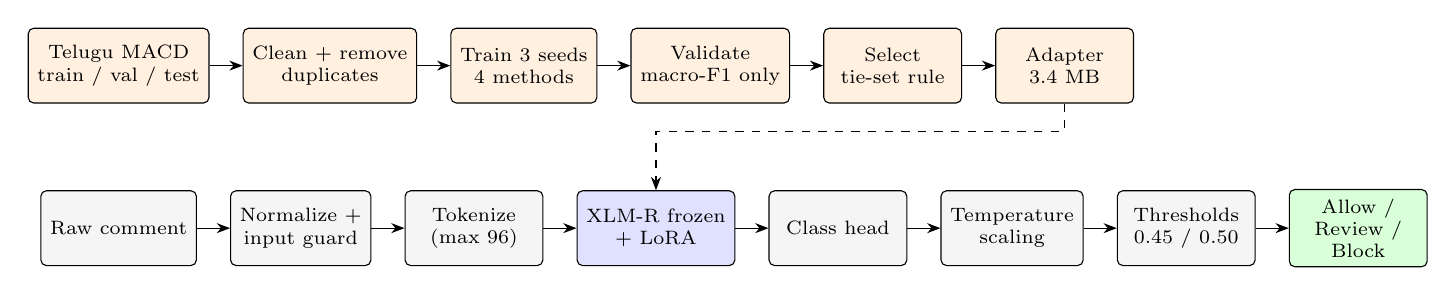
\begin{tikzpicture}[>=Stealth, node distance=0.42cm,
  block/.style={draw, rounded corners=2pt, align=center, font=\scriptsize, minimum height=0.95cm, minimum width=1.75cm, fill=gray!8},
  hlbox/.style={fill=blue!12}, outbox/.style={fill=green!15}, trbox/.style={fill=orange!12}]
% training path
\node[block, trbox] (d) {Telugu MACD\\train / val / test};
\node[block, trbox, right=of d] (c) {Clean + remove\\duplicates};
\node[block, trbox, right=of c] (t) {Train 3 seeds\\4 methods};
\node[block, trbox, right=of t] (v) {Validate\\macro-F1 only};
\node[block, trbox, right=of v] (s) {Select\\tie-set rule};
\node[block, trbox, right=of s] (ad) {Adapter\\3.4 MB};
\draw[->] (d)--(c); \draw[->] (c)--(t); \draw[->] (t)--(v); \draw[->] (v)--(s); \draw[->] (s)--(ad);
% inference path
\node[block, below=1.1cm of d] (r) {Raw comment};
\node[block, right=of r] (g) {Normalize +\\input guard};
\node[block, right=of g] (k) {Tokenize\\(max 96)};
\node[block, hlbox, right=of k] (e) {XLM-R frozen\\+ LoRA};
\node[block, right=of e] (h) {Class head};
\node[block, right=of h] (te) {Temperature\\scaling};
\node[block, right=of te] (th) {Thresholds\\0.45 / 0.50};
\node[block, outbox, right=of th] (o) {Allow /\\Review /\\Block};
\draw[->] (r)--(g); \draw[->] (g)--(k); \draw[->] (k)--(e); \draw[->] (e)--(h); \draw[->] (h)--(te); \draw[->] (te)--(th); \draw[->] (th)--(o);
\draw[->, dashed] (ad.south) -- ++(0,-0.35) -| (e.north);
\end{tikzpicture}}
\caption{Pipeline. Top: experiment and selection path (orange). Bottom: deployed inference path from raw comment to decision; the selected adapter (dashed arrow) is attached to the frozen encoder.}
\label{fig:arch}
\end{figure*}

\section{Results and Discussion}
\label{sec:results}
\subsection{Accuracy and cost}
Table~\ref{tab:main} reports mean and standard deviation over three seeds. Full fine-tuning, LoRA and DoRA on XLM-R and MuRIL lie between 0.9005 and 0.9057 test macro-F1, IndicBERT v2 LoRA reaches 0.9017 and mBERT LoRA 0.8946, and AdaLoRA is lowest (0.8891 on XLM-R, 0.8945 on MuRIL). The selected XLM-R LoRA model trains 887,042 parameters (0.32\% of 278.0 million) and peaks at 1.75~GB of GPU memory against 5.35~GB for full fine-tuning, with a 3.4~MB adapter in place of a 1.1~GB checkpoint. Figure~\ref{fig:front} plots accuracy against the number of trained parameters, and Fig.~\ref{fig:cost} compares memory and time.

\begin{table*}[t]
\caption{Test and validation macro-F1 (mean $\pm$ standard deviation, three seeds), trained parameters, peak GPU memory and training time. Selection used validation only. Times were measured with other load on the GPU and are indicative.}
\label{tab:main}
\centering
\footnotesize
\setlength{\tabcolsep}{5pt}
\begin{tabular}{llcccrrr}
\toprule
Backbone & Method & Val macro-F1 & Test macro-F1 & Trained params & GPU (GB) & Time (s) \\
\midrule
XLM-R & Full fine-tuning & $0.9040\pm0.0011$ & $0.9057\pm0.0033$ & 278.0 M & 5.35 & 1564 \\
XLM-R & LoRA (selected) & $0.9035\pm0.0043$ & $0.9035\pm0.0033$ & 0.887 M & 1.75 & 774 \\
XLM-R & DoRA & $0.9027\pm0.0011$ & $0.9055\pm0.0009$ & 0.905 M & 1.89 & 1125 \\
XLM-R & AdaLoRA & $0.8855\pm0.0015$ & $0.8891\pm0.0013$ & 1.035 M & 1.76 & 1618 \\
XLM-R & LoRA, $r{=}4,\alpha{=}32$, 5 ep.\ \cite{kaunang2026indo} & $0.8957\pm0.0014$ & $0.8985\pm0.0018$ & 0.740 M & 1.59 & 706 \\
XLM-R & LoRA, $r{=}16,\alpha{=}32$, 5 ep. & $0.8933\pm0.0002$ & $0.8953\pm0.0033$ & 1.182 M & 1.92 & 454 \\
MuRIL & Full fine-tuning & $0.9035\pm0.0023$ & $0.9049\pm0.0028$ & 237.6 M & 4.59 & 1250 \\
MuRIL & LoRA & $0.9026\pm0.0020$ & $0.9052\pm0.0030$ & 0.296 M & 1.59 & 718 \\
MuRIL & DoRA & $0.8984\pm0.0013$ & $0.9005\pm0.0030$ & 0.315 M & 1.73 & 1078 \\
MuRIL & AdaLoRA & $0.8892\pm0.0030$ & $0.8945\pm0.0003$ & 0.444 M & 1.60 & 1282 \\
IndicBERT v2 & LoRA & $0.8985\pm0.0014$ & $0.9017\pm0.0039$ & 0.296 M & 1.75 & 673 \\
mBERT & LoRA & $0.8999\pm0.0010$ & $0.8946\pm0.0015$ & 0.296 M & 1.37 & 680 \\
-- & TF-IDF + linear SVM (one run) & 0.8993 & 0.9029 & -- & CPU & -- \\
\bottomrule
\end{tabular}
\end{table*}

\begin{figure}[t]
\centering
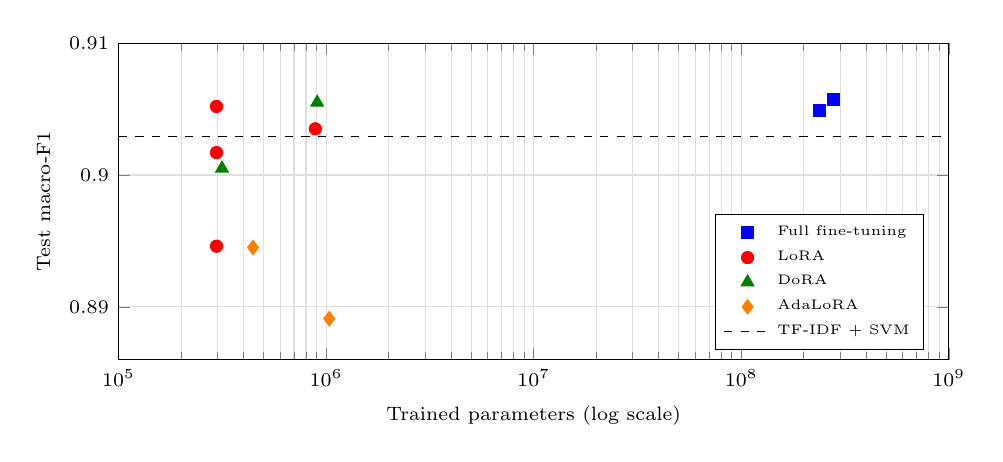
\begin{tikzpicture}
\begin{axis}[width=\columnwidth, height=5.6cm, xmode=log, xlabel={Trained parameters (log scale)}, ylabel={Test macro-F1},
  ymin=0.886, ymax=0.910, xmin=1e5, xmax=1e9, grid=both, grid style={gray!25},
  legend pos=south east, legend cell align=left]
\addplot[only marks, mark=square*, mark size=2.2pt, blue] coordinates {(278045186,0.9057) (237557762,0.9049)};
\addplot[only marks, mark=*, mark size=2.2pt, red] coordinates {(887042,0.9035) (296450,0.9052) (296450,0.9017) (296450,0.8946)};
\addplot[only marks, mark=triangle*, mark size=2.6pt, green!50!black] coordinates {(905474,0.9055) (314882,0.9005)};
\addplot[only marks, mark=diamond*, mark size=2.6pt, orange] coordinates {(1034786,0.8891) (444194,0.8945)};
\addplot[dashed, black, no markers] coordinates {(1e5,0.9029) (1e9,0.9029)};
\legend{Full fine-tuning, LoRA, DoRA, AdaLoRA, TF-IDF + SVM}
\end{axis}
\end{tikzpicture}
\caption{Test macro-F1 against trained parameters (mean of three seeds; XLM-R and MuRIL points; LoRA also shows IndicBERT v2 and mBERT). Almost all methods sit on one horizontal band, except AdaLoRA; the dashed line is the TF-IDF baseline.}
\label{fig:front}
\end{figure}

\begin{figure}[t]
\centering
\begin{minipage}{0.48\columnwidth}
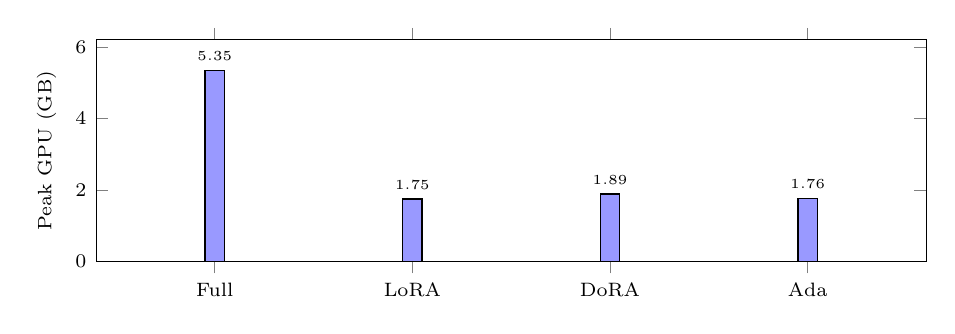
\begin{tikzpicture}
\begin{axis}[width=\linewidth, height=4.4cm, ybar, bar width=7pt, ymin=0, ymax=6.2, ylabel={Peak GPU (GB)},
  xtick={0,1,2,3}, xticklabels={Full,LoRA,DoRA,Ada}, nodes near coords, every node near coord/.append style={font=\tiny},
  enlarge x limits=0.2]
\addplot[fill=blue!40] coordinates {(0,5.35) (1,1.75) (2,1.89) (3,1.76)};
\end{axis}
\end{tikzpicture}
\end{minipage}\hfill
\begin{minipage}{0.48\columnwidth}
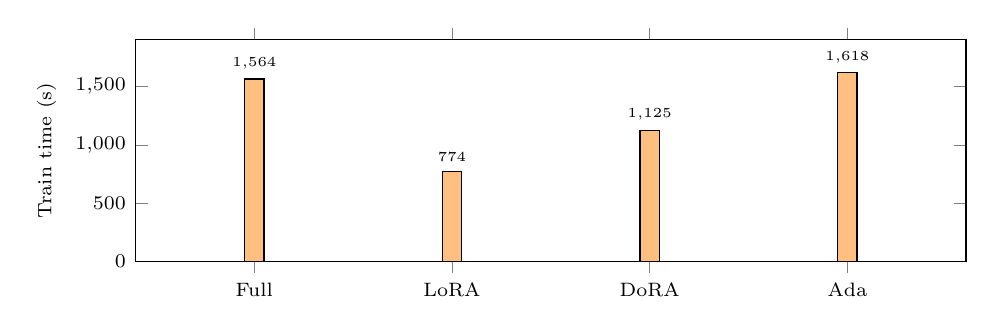
\begin{tikzpicture}
\begin{axis}[width=\linewidth, height=4.4cm, ybar, bar width=7pt, ymin=0, ymax=1900, ylabel={Train time (s)},
  xtick={0,1,2,3}, xticklabels={Full,LoRA,DoRA,Ada}, nodes near coords, every node near coord/.append style={font=\tiny},
  enlarge x limits=0.2]
\addplot[fill=orange!50] coordinates {(0,1564) (1,774) (2,1125) (3,1618)};
\end{axis}
\end{tikzpicture}
\end{minipage}
\caption{Cost on XLM-R (mean of three seeds). LoRA uses about one third of the memory of full fine-tuning; AdaLoRA is the slowest. Times include other GPU load and are indicative.}
\label{fig:cost}
\end{figure}

\subsection{Per-class metrics}
Table~\ref{tab:perclass} breaks the scores down by class. LoRA is more cautious than full fine-tuning: its precision on abusive comments is higher (0.929 against 0.914) but its recall is lower (0.883 against 0.905), so it misses more abuse and flags fewer innocent comments. Figure~\ref{fig:cm} shows the confusion matrix of the selected run. If missing abuse is the costlier error, full fine-tuning, DoRA, or a lower decision threshold on LoRA is the safer choice.

\begin{table*}[t]
\caption{Metrics averaged over three seeds on the test set. P and R are precision and recall for the abusive class.}
\label{tab:perclass}
\centering
\footnotesize
\setlength{\tabcolsep}{6pt}
\begin{tabular}{lccccccc}
\toprule
Model & Accuracy & P (abusive) & R (abusive) & F1 (abusive) & F1 (non-abusive) & Macro-F1 & Weighted-F1 \\
\midrule
XLM-R full fine-tuning & 0.906 & 0.914 & 0.905 & 0.909 & 0.902 & 0.906 & 0.906 \\
XLM-R LoRA (selected) & 0.904 & 0.929 & 0.883 & 0.905 & 0.902 & 0.904 & 0.904 \\
XLM-R DoRA & 0.906 & 0.922 & 0.894 & 0.908 & 0.903 & 0.906 & 0.906 \\
XLM-R AdaLoRA & 0.889 & 0.904 & 0.881 & 0.892 & 0.886 & 0.889 & 0.889 \\
MuRIL full fine-tuning & 0.905 & 0.919 & 0.897 & 0.908 & 0.902 & 0.905 & 0.905 \\
MuRIL LoRA & 0.905 & 0.919 & 0.898 & 0.908 & 0.902 & 0.905 & 0.905 \\
MuRIL DoRA & 0.901 & 0.913 & 0.895 & 0.904 & 0.897 & 0.900 & 0.901 \\
MuRIL AdaLoRA & 0.895 & 0.914 & 0.881 & 0.897 & 0.892 & 0.895 & 0.895 \\
IndicBERT v2 LoRA & 0.902 & 0.917 & 0.892 & 0.904 & 0.899 & 0.902 & 0.902 \\
mBERT LoRA & 0.895 & 0.917 & 0.877 & 0.897 & 0.893 & 0.895 & 0.895 \\
TF-IDF + linear SVM & 0.903 & 0.929 & 0.882 & 0.904 & 0.901 & 0.903 & 0.903 \\
\bottomrule
\end{tabular}
\end{table*}

\begin{figure}[t]
\centering
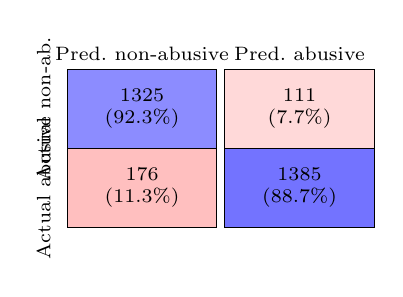
\begin{tikzpicture}[confcell/.style={minimum width=1.9cm, minimum height=1.0cm, draw, align=center, font=\scriptsize}]
\node[confcell, fill=blue!45] at (0,0) {1325\\(92.3\%)};
\node[confcell, fill=red!15] at (2,0) {111\\(7.7\%)};
\node[confcell, fill=red!25] at (0,-1) {176\\(11.3\%)};
\node[confcell, fill=blue!55] at (2,-1) {1385\\(88.7\%)};
\node[font=\scriptsize] at (0,0.7) {Pred.\ non-abusive};
\node[font=\scriptsize] at (2,0.7) {Pred.\ abusive};
\node[font=\scriptsize, rotate=90] at (-1.25,0) {Actual non-ab.};
\node[font=\scriptsize, rotate=90] at (-1.25,-1) {Actual abusive};
\end{tikzpicture}
\caption{Confusion matrix of the selected model (seed 2024) on 2,997 test comments; percentages are row-normalized.}
\label{fig:cm}
\end{figure}

\subsection{Where the models fail}
Table~\ref{tab:slices} reports test macro-F1 on slices of the test set for the selected model, full fine-tuning and the TF-IDF baseline (one seed each). Comments with emoji are the easiest (about 0.93). The transformers hold up better than TF-IDF on long comments of more than 20 words (0.902 and 0.911 against 0.887), which is consistent with their use of wider context, but the slices are small and single-seed, so these differences are indicative only.

\begin{table}[t]
\caption{Test macro-F1 on slices of the test set (one seed per system). ``Latin letters'' marks comments with any Roman-script character.}
\label{tab:slices}
\centering
\footnotesize
\setlength{\tabcolsep}{4pt}
\begin{tabular}{lrcccc}
\toprule
Slice & $n$ & Abusive & LoRA & Full FT & TF-IDF \\
\midrule
1--5 words & 814 & 0.40 & 0.897 & 0.900 & 0.901 \\
6--10 words & 976 & 0.47 & 0.903 & 0.910 & 0.907 \\
11--20 words & 729 & 0.59 & 0.894 & 0.898 & 0.888 \\
Over 20 words & 478 & 0.73 & 0.902 & 0.911 & 0.887 \\
Contains emoji & 1,178 & 0.53 & 0.929 & 0.934 & 0.925 \\
Contains Latin letters & 616 & 0.65 & 0.910 & 0.900 & 0.908 \\
Telugu script only & 2,381 & 0.49 & 0.901 & 0.910 & 0.900 \\
\bottomrule
\end{tabular}
\end{table}

The errors are strongly shared. Comparing single runs (seed 2024 for the transformers), of the 287 test errors of the selected model, 122 (42.5\%) are also made by full fine-tuning, DoRA, MuRIL LoRA and TF-IDF; 86 of these 122 carry the abusive label and 36 the non-abusive label. The selected model's errors overlap with those of full fine-tuning (Jaccard 0.60) more than with those of TF-IDF (0.45). Had at least one of the five systems been chosen correctly for every comment, accuracy would be 0.959, an upper bound that suggests some room for combining models. The selected model misses abuse more often than it raises false alarms (178 false negatives against 112 false positives after calibration and the input guard), and 101 of its 290 errors in the deployed pipeline have a confidence of at least 0.9. Comments that every system gets wrong with high confidence are candidates for label noise or for abuse that needs context; they were not re-annotated.

\subsection{Template artifacts in the data}
The word-frequency analysis of the training split showed a group of terms that occur almost only in abusive comments and are not abusive words: the Telugu words for ``problems'', ``for any problem'', ``progeny'', ``husband and wife'', a term for love spells, and formal phrases such as ``will be done''. They come from advertisement-like posts for astrology and spell services. Every comment containing one of these markers was flagged (Table~\ref{tab:template}). About 15\% of abusive comments in each split are such posts, and almost all flagged posts carry the abusive label. All three systems classify them with 99.6\% accuracy. Removing them from the test set lowers macro-F1 by about 0.7 to 0.8 points for every system (seed 2024; selected LoRA 0.8964, full fine-tuning 0.9019, TF-IDF 0.8949), so the comparison between systems does not change, but reported scores on this corpus are inflated by an easy, template-driven subset. Whether such posts should count as abusive is a labeling decision of the source corpus, which was not revisited.

\begin{table}[t]
\caption{Advertisement-like template posts flagged by seven marker strings.}
\label{tab:template}
\centering
\footnotesize
\setlength{\tabcolsep}{4pt}
\begin{tabular}{lrrrr}
\toprule
Split & Flagged & Labeled abusive & Labeled non-abusive & Share of abusive \\
\midrule
Train & 1,935 & 1,928 & 7 & 15.5\% \\
Validation & 267 & 264 & 3 & 16.3\% \\
Test & 227 & 227 & 0 & 14.5\% \\
\bottomrule
\end{tabular}
\end{table}

\subsection{Training behavior}
Figure~\ref{fig:curve} shows validation macro-F1 per epoch for the selected seed. LoRA peaks at epoch 6 and early stopping ends training at epoch 9, while full fine-tuning reaches its best score at epoch 4. LoRA needs more epochs than full fine-tuning here; a likely reason is that only a small number of parameters move at each step, but this was not tested.

\begin{figure}[t]
\centering
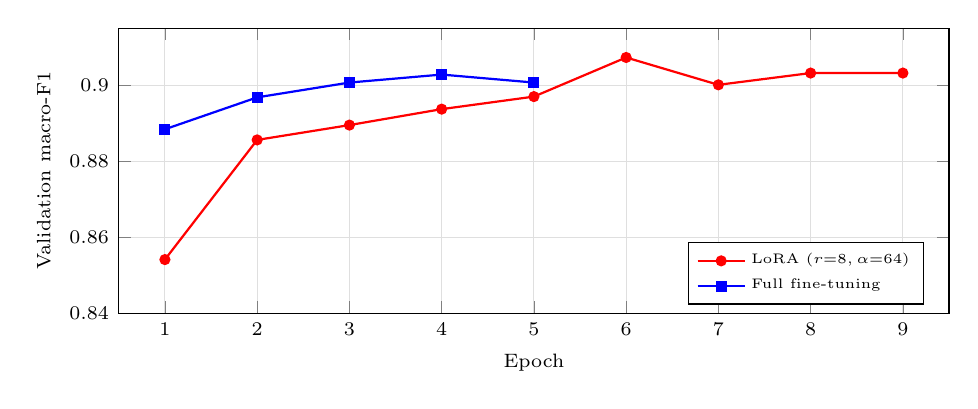
\begin{tikzpicture}
\begin{axis}[width=\columnwidth, height=5.2cm, xlabel={Epoch}, ylabel={Validation macro-F1}, ymin=0.84, ymax=0.915, xmin=0.5, xmax=9.5,
  grid=both, grid style={gray!25}, legend pos=south east, legend cell align=left, xtick={1,...,9}]
\addplot[red, thick, mark=*, mark size=1.6pt] coordinates {(1,0.8541) (2,0.8856) (3,0.8895) (4,0.8937) (5,0.8970) (6,0.9073) (7,0.9001) (8,0.9032) (9,0.9032)};
\addplot[blue, thick, mark=square*, mark size=1.6pt] coordinates {(1,0.8884) (2,0.8968) (3,0.9007) (4,0.9028) (5,0.9007)};
\addlegendentry{LoRA ($r{=}8,\alpha{=}64$)}
\addlegendentry{Full fine-tuning}
\end{axis}
\end{tikzpicture}
\caption{Validation macro-F1 per epoch for XLM-R, seed 2024. Both curves flatten within about one point of each other.}
\label{fig:curve}
\end{figure}

\subsection{Rank, alpha and learning rate}
Table~\ref{tab:grid} shows the MuRIL grid (one seed). The whole grid spans about 1.5 points on validation, which is of the same order as seed-to-seed variation, so no single rank can be called best with confidence. Alpha~$=64$ was best at every rank. A learning rate of $10^{-4}$ under-trained (validation 0.8922) and $5\times10^{-4}$ degraded training (0.8438), against 0.9048 at $2\times10^{-4}$.

\begin{table}[t]
\caption{Validation macro-F1 on MuRIL for LoRA rank $r$ and alpha $\alpha$ (learning rate $2\times10^{-4}$, one seed). Bold is the best cell.}
\label{tab:grid}
\centering
\footnotesize
\begin{tabular}{lccc}
\toprule
 & $\alpha=16$ & $\alpha=32$ & $\alpha=64$ \\
\midrule
$r=4$ & 0.8896 & 0.8978 & 0.9002 \\
$r=8$ & 0.8915 & 0.8978 & \textbf{0.9048} \\
$r=16$ & 0.8982 & 0.8957 & 0.9006 \\
$r=32$ & 0.8944 & 0.8973 & 0.9019 \\
\bottomrule
\end{tabular}
\end{table}

\subsection{Significance}
Table~\ref{tab:sig} and Fig.~\ref{fig:forest} compare the selected XLM-R LoRA model with each alternative on the same test comments. Against full fine-tuning the interval includes zero for all three seeds (McNemar $p$ between 0.24 and 0.87), and the same holds for DoRA, MuRIL LoRA, MuRIL full fine-tuning, IndicBERT v2, the published recipe and the TF-IDF baseline. AdaLoRA is worse by 0.016 macro-F1 ($p=0.0002$). mBERT is worse with an interval that just excludes zero but a McNemar $p$ of 0.054. A seed-level Welch test of LoRA against full fine-tuning gives $p=0.47$ with three seeds per arm, which has little power. The test set of 2,997 comments cannot resolve differences much below one point, so the supported statement is non-inferiority within about one point, not superiority.

\begin{table}[t]
\caption{Selected XLM-R LoRA (seed 2024) minus each alternative on 2,997 test comments: macro-F1 difference, 95\% paired bootstrap interval and exact McNemar $p$.}
\label{tab:sig}
\centering
\footnotesize
\setlength{\tabcolsep}{3.5pt}
\begin{tabular}{lccc}
\toprule
Alternative & $\Delta$ & 95\% interval & $p$ \\
\midrule
XLM-R full, seed 2024 & $-0.0050$ & $[-0.0127,+0.0027]$ & 0.235 \\
XLM-R full, seed 42 & $-0.0009$ & $[-0.0091,+0.0074]$ & 0.872 \\
XLM-R full, seed 123 & $+0.0015$ & $[-0.0067,+0.0095]$ & 0.811 \\
XLM-R DoRA & $-0.0004$ & $[-0.0070,+0.0063]$ & 1.000 \\
MuRIL LoRA & $+0.0024$ & $[-0.0060,+0.0107]$ & 0.634 \\
MuRIL full & $-0.0007$ & $[-0.0097,+0.0080]$ & 0.941 \\
Published recipe & $+0.0037$ & $[-0.0037,+0.0107]$ & 0.355 \\
IndicBERT v2 LoRA & $+0.0067$ & $[-0.0024,+0.0157]$ & 0.168 \\
TF-IDF + SVM & $+0.0013$ & $[-0.0084,+0.0110]$ & 0.840 \\
mBERT LoRA & $+0.0097$ & $[+0.0007,+0.0193]$ & 0.054 \\
XLM-R AdaLoRA & $+0.0160$ & $[+0.0077,+0.0244]$ & 0.0002 \\
\bottomrule
\end{tabular}
\end{table}

\begin{figure}[t]
\centering
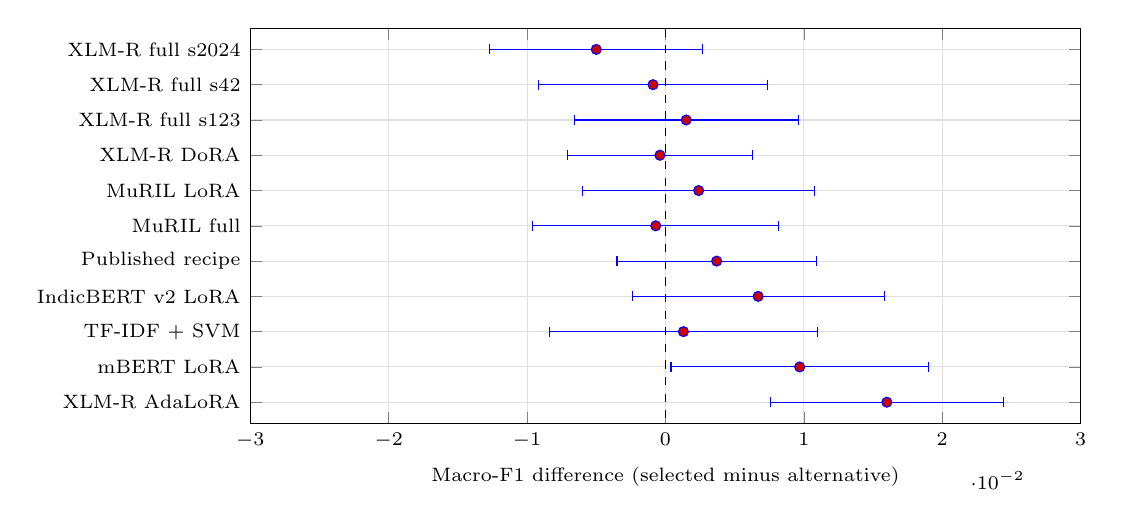
\begin{tikzpicture}
\begin{axis}[width=\columnwidth, height=6.6cm, xlabel={Macro-F1 difference (selected minus alternative)}, xmin=-0.03, xmax=0.03,
  y dir=reverse, ymin=0.4, ymax=11.6, ytick={1,...,11},
  yticklabels={XLM-R full s2024,XLM-R full s42,XLM-R full s123,XLM-R DoRA,MuRIL LoRA,MuRIL full,Published recipe,IndicBERT v2 LoRA,TF-IDF + SVM,mBERT LoRA,XLM-R AdaLoRA},
  grid=major, grid style={gray!25}]
\addplot[black, dashed, no markers] coordinates {(0,0.4) (0,11.6)};
\addplot+[only marks, mark=*, mark size=1.8pt, blue, error bars/.cd, x dir=both, x explicit]
  coordinates {(-0.0050,1) +- (0.0077,0) (-0.0009,2) +- (0.0083,0) (0.0015,3) +- (0.0081,0) (-0.0004,4) +- (0.0067,0)
  (0.0024,5) +- (0.0084,0) (-0.0007,6) +- (0.0089,0) (0.0037,7) +- (0.0072,0) (0.0067,8) +- (0.0091,0)
  (0.0013,9) +- (0.0097,0) (0.0097,10) +- (0.0093,0) (0.0160,11) +- (0.0084,0)};
\end{axis}
\end{tikzpicture}
\caption{Paired macro-F1 difference between the selected model and each alternative with 95\% bootstrap intervals (dashed line: no difference; right of zero favours the selected model). Only AdaLoRA, and marginally mBERT, are clearly separated.}
\label{fig:forest}
\end{figure}

\subsection{Expected versus observed outcomes}
Table~\ref{tab:expect} summarizes the expected and observed outcome for each model. Several expected benefits did not appear. AdaLoRA was expected to improve on uniform rank allocation, but it was the weakest method on both backbones and took about twice the training time of LoRA; an earlier run collapsed to chance level before its rank-allocation step was corrected, so this method is sensitive to implementation details. DoRA was expected to help especially at low rank, but gave a tie on XLM-R and a lower score on MuRIL. Indic-specific pretraining (MuRIL, IndicBERT v2) did not beat XLM-R. The published recipe transferred but scored 0.8985, about 0.5 points below the tuned setting; since rank, alpha, dropout, batch size, length and epoch budget all differ, the gap cannot be attributed to one factor, and two of three seeds of the $r=16$ configuration peaked on the last allowed epoch, which suggests that five epochs is short.

\begin{table*}[t]
\caption{Expectation against outcome for each model tested (test macro-F1, mean over seeds).}
\label{tab:expect}
\centering
\footnotesize
\begin{tabular}{>{\raggedright\arraybackslash}p{2.8cm}>{\raggedright\arraybackslash}p{4.8cm}>{\raggedright\arraybackslash}p{6.0cm}>{\raggedright\arraybackslash}p{2.2cm}}
\toprule
Model & Expected & Observed & Verdict \\
\midrule
XLM-R full fine-tuning & Accuracy ceiling & 0.9057, tied with cheaper models & Met as baseline \\
XLM-R LoRA & Near full accuracy with 1--2\% of the weights \cite{kaunang2026indo} & 0.9035 with 0.32\% of the weights & Met \\
LoRA rank study & A clear best rank & Rank barely matters, alpha does & Partly not met \\
AdaLoRA & Better than LoRA \cite{zhang2023adalora} & 0.8891, worse ($p=0.0002$), 2$\times$ slower & Not met \\
DoRA & Better than LoRA \cite{liu2024dora} & 0.9055 on XLM-R (tie), 0.9005 on MuRIL (lower) & Not met \\
mBERT LoRA & Trails XLM-R & 0.8946, the lowest backbone & Met \\
IndicBERT v2 LoRA & Beats general models on Telugu & 0.9017, tied, no gain & Not met \\
MuRIL & Beats XLM-R on Telugu & 0.9049 / 0.9052 vs 0.9057 / 0.9035, tied & Not met \\
Published recipe & Near optimal & 0.8985, slightly lower & Partly not met \\
TF-IDF + SVM & Floor well below transformers & 0.9029, statistically tied & Not met \\
INT8 export & Small loss \cite{jacob2018} & Per-tensor collapsed; per-channel loses 1.2 points & Failed, then fixed \\
\bottomrule
\end{tabular}
\end{table*}

\subsection{Comparison with the classical baseline}
The TF-IDF and linear SVM model reaches 0.9029 test macro-F1 with a 30.3~MB file and a median latency of 1.65~ms per comment on one CPU thread, and it is statistically indistinguishable from the selected model ($p=0.84$). On this corpus, therefore, the transformers do not buy accuracy; the finding of this study is that adapting them cheaply costs no accuracy. It was not tested whether transformers help on implicit abuse, unseen vocabulary or code-mixed text, which is where an advantage would be expected.

\subsection{Robustness to disguised text}
The robustness experiment applies seven sentence-level and thirteen per-word disguises (spacing, zero-width characters, repeated letters, emoji, leetspeak, star-censoring, case) to 600 test comments. Without the input guard, every system drops to a mean accuracy of about 0.71 (Table~\ref{tab:rob} and Fig.~\ref{fig:rob}). With the guard, all three systems reach 0.86, so the gain comes from the guard and not from the model. Star-censored words (about 0.55) and combined letter repetition with zero-width characters remain weak points for all systems.

\begin{table}[t]
\caption{Accuracy on 600 test comments under 20 disguise attacks, with and without the input guard.}
\label{tab:rob}
\centering
\footnotesize
\setlength{\tabcolsep}{4pt}
\begin{tabular}{lccc}
\toprule
System & Clean & Mean attack & Worst attack \\
\midrule
TF-IDF + SVM, no guard & 0.910 & 0.712 & 0.450 \\
XLM-R full, no guard & 0.907 & 0.710 & 0.455 \\
XLM-R LoRA, no guard & 0.897 & 0.725 & 0.458 \\
XLM-R LoRA + guard & 0.898 & 0.856 & 0.552 \\
XLM-R full + guard & 0.907 & 0.860 & 0.550 \\
TF-IDF + SVM + guard & 0.910 & 0.863 & 0.560 \\
\bottomrule
\end{tabular}
\end{table}

\begin{figure}[t]
\centering
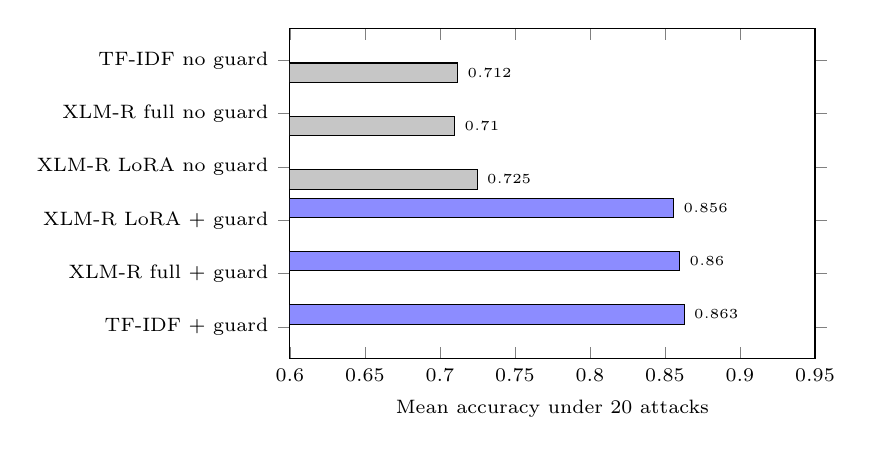
\begin{tikzpicture}
\begin{axis}[width=0.55\columnwidth, scale only axis, height=4.2cm, xbar, bar width=7pt, xmin=0.6, xmax=0.95, xlabel={Mean accuracy under 20 attacks},
  y dir=reverse, ytick={0,...,5},
  yticklabels={TF-IDF no guard,XLM-R full no guard,XLM-R LoRA no guard,XLM-R LoRA + guard,XLM-R full + guard,TF-IDF + guard},
  nodes near coords={\pgfmathprintnumber[fixed,precision=3]{\pgfplotspointmeta}}, every node near coord/.append style={font=\tiny},
  enlarge y limits=0.12]
\addplot[fill=gray!45] coordinates {(0.712,0) (0.710,1) (0.725,2)};
\addplot[fill=blue!45] coordinates {(0.856,3) (0.860,4) (0.863,5)};
\end{axis}
\end{tikzpicture}
\caption{Mean accuracy under disguise attacks. The three guarded systems (blue) are far above the unguarded ones (grey) and are indistinguishable from each other.}
\label{fig:rob}
\end{figure}

Table~\ref{tab:attacks} breaks the robustness result down by attack. The guard repairs zero-width characters and separators inside words almost completely, partly repairs letter spacing and repetition, and cannot help with star-censoring, which removes the letters themselves. Emoji-based disguises are the one place where the model matters: without any guard-related repair, the selected LoRA model keeps 0.89 to 0.90 accuracy when words are wrapped in emoji or followed by emoji spam, against 0.80 to 0.85 for TF-IDF and 0.82 to 0.84 for full fine-tuning. Both transformers use the same inference code, so this difference originates in the models; the cause of the lower emoji sensitivity of the adapted model remains to be investigated.

\begin{table*}[t]
\caption{Accuracy on 600 test comments for each attack, without / with the input guard. Sentence-level attacks change the whole comment; per-word attacks change every word.}
\label{tab:attacks}
\centering
\footnotesize
\setlength{\tabcolsep}{6pt}
\begin{tabular}{llccc}
\toprule
Level & Attack & TF-IDF + SVM & XLM-R full FT & XLM-R LoRA (selected) \\
\midrule
-- & None (clean) & 0.910 / 0.910 & 0.907 / 0.907 & 0.897 / 0.898 \\
Sentence & Repeated characters & 0.832 / 0.882 & 0.778 / 0.870 & 0.767 / 0.862 \\
Sentence & Extra spacing & 0.790 / 0.873 & 0.775 / 0.887 & 0.763 / 0.863 \\
Sentence & Emoji inserted & 0.892 / 0.892 & 0.902 / 0.902 & 0.902 / 0.903 \\
Sentence & Punctuation inserted & 0.893 / 0.895 & 0.908 / 0.908 & 0.897 / 0.897 \\
Sentence & Capitalization & 0.910 / 0.910 & 0.908 / 0.908 & 0.902 / 0.902 \\
Sentence & Number substitution & 0.903 / 0.905 & 0.912 / 0.912 & 0.890 / 0.893 \\
Sentence & Random case & 0.910 / 0.910 & 0.908 / 0.908 & 0.897 / 0.898 \\
Word & Zero-width joiner & 0.688 / 0.910 & 0.455 / 0.907 & 0.458 / 0.898 \\
Word & Zero-width non-joiner & 0.450 / 0.910 & 0.455 / 0.907 & 0.458 / 0.898 \\
Word & Letter spacing & 0.608 / 0.835 & 0.455 / 0.845 & 0.458 / 0.765 \\
Word & Dots between letters & 0.477 / 0.893 & 0.508 / 0.902 & 0.480 / 0.890 \\
Word & Dashes between letters & 0.453 / 0.890 & 0.487 / 0.897 & 0.515 / 0.888 \\
Word & Emoji inside word & 0.460 / 0.892 & 0.655 / 0.900 & 0.758 / 0.905 \\
Word & Emoji wrapped around word & 0.800 / 0.800 & 0.818 / 0.818 & 0.890 / 0.892 \\
Word & Repeated characters & 0.493 / 0.820 & 0.570 / 0.775 & 0.643 / 0.758 \\
Word & Leetspeak digits & 0.903 / 0.905 & 0.907 / 0.907 & 0.893 / 0.895 \\
Word & Star-censored & 0.558 / 0.560 & 0.550 / 0.550 & 0.552 / 0.552 \\
Word & Uppercase & 0.910 / 0.910 & 0.908 / 0.908 & 0.897 / 0.898 \\
Word & Trailing emoji spam & 0.852 / 0.852 & 0.837 / 0.837 & 0.900 / 0.902 \\
Word & Combined (repeat, zero-width, emoji) & 0.452 / 0.822 & 0.507 / 0.757 & 0.572 / 0.758 \\
\bottomrule
\end{tabular}
\end{table*}

\subsection{Calibration, thresholds and deployment}
Temperature scaling (T = 1.334) reduces the expected calibration error of the selected model on validation from 0.035 to 0.013 and the Brier score from 0.0730 to 0.0711. With thresholds 0.45 and 0.50, the block decision has precision 0.928 and recall 0.897 on validation and sends 1.1\% of comments to human review. Table~\ref{tab:dep} shows the deployment variants. The INT8 export with per-channel weights loses about 1.2 points of test macro-F1 relative to FP32 and agrees with it on 96.8\% of test predictions. A per-tensor INT8 export of the MuRIL LoRA model made earlier in the study collapsed to 0.633 test macro-F1, and an INT8 file produced earlier in this project with the same per-tensor recipe scored 0.37 on a 600-comment sample; these failures would have gone unnoticed without evaluating the quantized model against FP32.

\begin{table}[t]
\caption{Deployment variants of the selected model. Latency is the median per comment including tokenization, batch size one, on the development PC.}
\label{tab:dep}
\centering
\footnotesize
\setlength{\tabcolsep}{3pt}
\begin{tabular}{lccccc}
\toprule
Variant & Size & Val F1 & Test F1 & 1 thr. & 4 thr. \\
\midrule
FP32 merged (PyTorch) & 1.1 GB & 0.9073 & 0.9042 & 43.1 ms & 17.9 ms \\
INT8 ONNX, per-channel & 279 MB & 0.8995 & 0.8926 & 23.1 ms & 8.3 ms \\
TF-IDF + SVM & 30.3 MB & 0.8993 & 0.9029 & 1.65 ms & -- \\
\bottomrule
\end{tabular}
\end{table}

Figure~\ref{fig:calib} shows the reliability of the scores and the trade-off behind the thresholds. Before scaling, the model is over-confident: comments scored between 0.8 and 0.9 are right only 77\% of the time; after scaling, 82\%. Raising the block threshold trades recall for precision and sends more comments to review: at 0.70 the block precision is 0.950, recall 0.855 and 4.7\% of comments go to review; at 0.90 the figures are 0.984, 0.760 and 11.6\%. The chosen 0.50 keeps human review to about 1\% of traffic.

\begin{figure}[t]
\centering
\begin{minipage}{0.49\columnwidth}
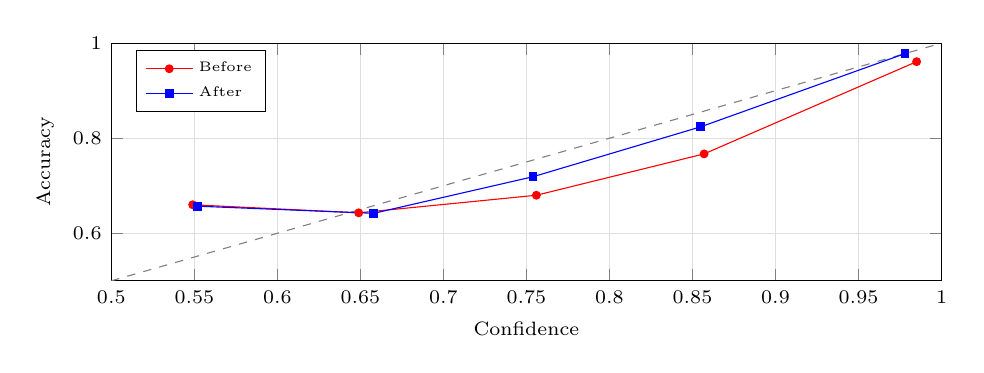
\begin{tikzpicture}
\begin{axis}[width=\linewidth, height=4.6cm, xmin=0.5, xmax=1, ymin=0.5, ymax=1, xlabel={Confidence}, ylabel={Accuracy},
  grid=both, grid style={gray!25}, legend pos=north west, legend cell align=left]
\addplot[gray, dashed, no markers, forget plot] coordinates {(0.5,0.5) (1,1)};
\addplot[red, mark=*, mark size=1.4pt] coordinates {(0.549,0.660) (0.649,0.643) (0.756,0.680) (0.857,0.767) (0.985,0.961)};
\addplot[blue, mark=square*, mark size=1.4pt] coordinates {(0.552,0.657) (0.658,0.642) (0.754,0.719) (0.855,0.824) (0.978,0.978)};
\addlegendentry{Before}
\addlegendentry{After}
\end{axis}
\end{tikzpicture}
\end{minipage}\hfill
\begin{minipage}{0.49\columnwidth}
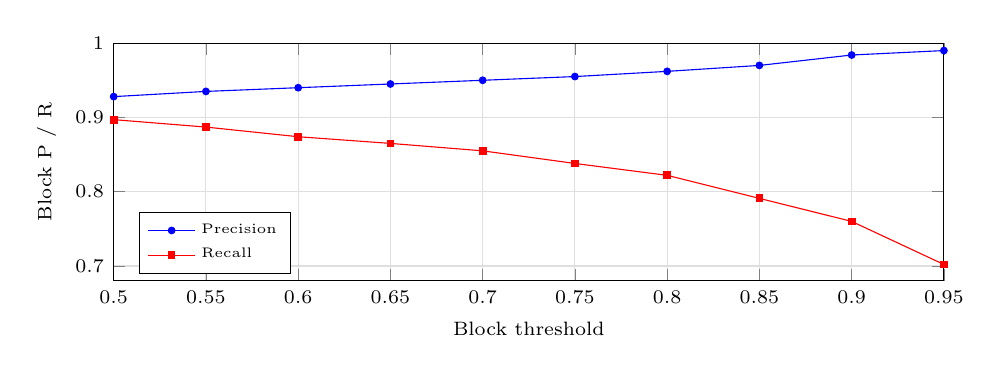
\begin{tikzpicture}
\begin{axis}[width=\linewidth, height=4.6cm, xmin=0.5, xmax=0.95, ymin=0.68, ymax=1, xlabel={Block threshold}, ylabel={Block P / R},
  grid=both, grid style={gray!25}, legend pos=south west, legend cell align=left]
\addplot[blue, mark=*, mark size=1.2pt] coordinates {(0.50,0.928) (0.55,0.935) (0.60,0.940) (0.65,0.945) (0.70,0.950) (0.75,0.955) (0.80,0.962) (0.85,0.970) (0.90,0.984) (0.95,0.990)};
\addplot[red, mark=square*, mark size=1.2pt] coordinates {(0.50,0.897) (0.55,0.887) (0.60,0.874) (0.65,0.865) (0.70,0.855) (0.75,0.838) (0.80,0.822) (0.85,0.791) (0.90,0.760) (0.95,0.702)};
\addlegendentry{Precision}
\addlegendentry{Recall}
\end{axis}
\end{tikzpicture}
\end{minipage}
\caption{Left: reliability on validation before and after temperature scaling (points on the dashed line are perfectly calibrated). Right: precision and recall of the block decision as the block threshold rises, with the review threshold fixed at 0.45.}
\label{fig:calib}
\end{figure}

\subsection{Deployment recommendations}
Table~\ref{tab:choose} turns the results into a choice. The evidence supports using a LoRA adapter when a transformer is wanted, and a TF-IDF model with the input guard when the smallest and fastest system is wanted; the guard should be kept in both cases.

\begin{table}[t]
\caption{Recommended choice by requirement.}
\label{tab:choose}
\centering
\footnotesize
\begin{tabular}{>{\raggedright\arraybackslash}p{2.7cm}>{\raggedright\arraybackslash}p{1.9cm}>{\raggedright\arraybackslash}p{3.1cm}}
\toprule
Requirement & Choice & Reason \\
\midrule
Smallest, fastest, CPU only & TF-IDF + SVM + guard & 30 MB, about 2 ms, same accuracy \\
A transformer with a tiny file & XLM-R + LoRA & 3.4 MB adapter, one third of the memory \\
Catch as much abuse as possible & Full FT or DoRA, or lower threshold & Higher abusive recall \\
Never use & Per-tensor INT8 & Collapsed to 0.63 macro-F1 \\
\bottomrule
\end{tabular}
\end{table}

\subsection{Lessons for practitioners}
Three problems in this project changed the conclusions until they were found. First, an earlier run of LoRA with learning rate $10^{-4}$, three epochs and no early stopping gave 0.868 test macro-F1 on MuRIL and suggested that PEFT trails full fine-tuning by about four points; with learning rate $2\times10^{-4}$ and up to ten epochs the gap disappeared. Second, AdaLoRA first collapsed to 0.34 macro-F1; its rank-allocation step had never been called during training and its schedule was hard-coded, and fixing both (together with the new learning-rate setting) restored it to 0.89. Third, the per-tensor INT8 export scored 0.37 to 0.63 while looking like a normal model file. In each case the remedy was the same: compare against a trusted reference before drawing a conclusion. A short learning-rate and epoch search, a check that method-specific training hooks run, and an accuracy check of every exported model are cheap and would have prevented all three.

\subsection{Threats to validity}
The study uses one dataset in one language and a single test set of 2,997 comments. Three seeds give only coarse variance estimates, and the rank, alpha and learning-rate searches used one seed on MuRIL. Hyperparameters tuned for LoRA were reused for DoRA and AdaLoRA, which may understate them. Robustness was measured on 600 comments with synthetic disguises and may not reflect real attacks. Latency was measured on a desktop PC and not on low-end laptops, and peak RAM was not measured. Comments contain real abusive text; the corpus labels are those of the source dataset and were not re-annotated.

\subsection{Ethical considerations and reproducibility}
The system is meant to assist human moderators, not to replace them: the review band exists because about one test comment in ten is misclassified and false positives on critical or political speech carry real costs. The corpus contains real abusive text, which was used only as released, without new annotation or contact with users; examples are not reproduced in this paper. For reproducibility, every configuration was run with fixed seeds, all per-run metrics, training logs and confusion matrices were kept, and the selection rule is fully specified (Fig.~\ref{alg:select}). The study needs one 8~GB consumer GPU; the 50 training runs of the study took about 12.6 hours of training time in total.

\section{Conclusion and Future Work}
\label{sec:concl}
On Telugu abusive comment detection, LoRA on the query and value matrices matches full fine-tuning within statistical noise while training under one percent of the parameters and using about a third of the GPU memory, so a 3.4~MB adapter can replace a 1.1~GB checkpoint. DoRA and AdaLoRA bring no benefit here, Indic-specific backbones do not beat XLM-R, and a TF-IDF and linear SVM baseline is as accurate on this corpus. The robustness measured here comes mostly from a simple input guard, although the adapted model is clearly less sensitive to emoji-based disguises. About 15\% of abusive comments are advertisement-like templates that inflate all scores, and 42\% of the selected model's errors are shared by every strong system. The most serious deployment error found was a silently broken INT8 export. Future work should evaluate on code-mixed and Romanized Telugu and on other domains where contextual models may help, tune DoRA and AdaLoRA separately, run more seeds and a larger test set, measure latency and memory on low-end laptops, test learned rather than rule-based defenses against disguised text, re-annotate the comments that every system misclassifies, and report scores with and without template posts.

\begin{thebibliography}{00}
\bibitem{kaunang2026indo} F. J. Kaunang, B. Hakim, and A. P. Thenata, ``Indonesian hate speech detection across diverse domains using parameter-efficient fine-tuning with IndoBERT and LoRA,'' \textit{Jurnal Minfo Polgan}, vol. 15, no. 2, 2026, doi:10.33395/jmp.v15i2.16581.
\bibitem{gupta2022macd} V. Gupta \textit{et al.}, ``Multilingual abusive comment detection at scale for Indic languages,'' in \textit{Advances in Neural Information Processing Systems 35, Datasets and Benchmarks Track}, 2022.
\bibitem{waseem2016} Z. Waseem and D. Hovy, ``Hateful symbols or hateful people? Predictive features for hate speech detection on Twitter,'' in \textit{Proc. NAACL Student Research Workshop}, 2016, pp. 88--93.
\bibitem{davidson2017} T. Davidson, D. Warmsley, M. Macy, and I. Weber, ``Automated hate speech detection and the problem of offensive language,'' in \textit{Proc. Int. AAAI Conf. Web and Social Media (ICWSM)}, vol. 11, no. 1, 2017, pp. 512--515.
\bibitem{schmidt2017} A. Schmidt and M. Wiegand, ``A survey on hate speech detection using natural language processing,'' in \textit{Proc. Fifth Int. Workshop on Natural Language Processing for Social Media}, 2017, pp. 1--10.
\bibitem{vaswani2017} A. Vaswani \textit{et al.}, ``Attention is all you need,'' in \textit{Advances in Neural Information Processing Systems 30}, 2017.
\bibitem{houlsby2019} N. Houlsby \textit{et al.}, ``Parameter-efficient transfer learning for NLP,'' in \textit{Proc. 36th Int. Conf. Machine Learning (ICML)}, PMLR vol. 97, 2019, pp. 2790--2799.
\bibitem{li2021prefix} X. L. Li and P. Liang, ``Prefix-tuning: Optimizing continuous prompts for generation,'' in \textit{Proc. 59th Annu. Meeting Assoc. Computational Linguistics (ACL)}, 2021, pp. 4582--4597.
\bibitem{lester2021prompt} B. Lester, R. Al-Rfou, and N. Constant, ``The power of scale for parameter-efficient prompt tuning,'' in \textit{Proc. Conf. Empirical Methods in Natural Language Processing (EMNLP)}, 2021, pp. 3045--3059.
\bibitem{aghajanyan2021intrinsic} A. Aghajanyan, S. Gupta, and L. Zettlemoyer, ``Intrinsic dimensionality explains the effectiveness of language model fine-tuning,'' in \textit{Proc. 59th Annu. Meeting Assoc. Computational Linguistics (ACL)}, 2021, pp. 7319--7328.
\bibitem{hu2022lora} E. J. Hu \textit{et al.}, ``LoRA: Low-rank adaptation of large language models,'' in \textit{Proc. Int. Conf. Learning Representations (ICLR)}, 2022.
\bibitem{zhang2023adalora} Q. Zhang \textit{et al.}, ``Adaptive budget allocation for parameter-efficient fine-tuning,'' in \textit{Proc. Int. Conf. Learning Representations (ICLR)}, 2023.
\bibitem{liu2024dora} S.-Y. Liu \textit{et al.}, ``DoRA: Weight-decomposed low-rank adaptation,'' in \textit{Proc. 41st Int. Conf. Machine Learning (ICML)}, PMLR vol. 235, 2024.
\bibitem{dettmers2023qlora} T. Dettmers, A. Pagnoni, A. Holtzman, and L. Zettlemoyer, ``QLoRA: Efficient finetuning of quantized LLMs,'' in \textit{Advances in Neural Information Processing Systems 36}, 2023.
\bibitem{liu2022ia3} H. Liu \textit{et al.}, ``Few-shot parameter-efficient fine-tuning is better and cheaper than in-context learning,'' in \textit{Advances in Neural Information Processing Systems 35}, 2022.
\bibitem{mangrulkar2022peft} S. Mangrulkar \textit{et al.}, ``PEFT: State-of-the-art parameter-efficient fine-tuning methods,'' 2022. [Online]. Available: \url{https://github.com/huggingface/peft}
\bibitem{conneau2020xlmr} A. Conneau \textit{et al.}, ``Unsupervised cross-lingual representation learning at scale,'' in \textit{Proc. 58th Annu. Meeting Assoc. Computational Linguistics (ACL)}, 2020, pp. 8440--8451.
\bibitem{khanuja2021muril} S. Khanuja \textit{et al.}, ``MuRIL: Multilingual representations for Indian languages,'' arXiv:2103.10730, 2021.
\bibitem{devlin2019bert} J. Devlin, M.-W. Chang, K. Lee, and K. Toutanova, ``BERT: Pre-training of deep bidirectional transformers for language understanding,'' in \textit{Proc. NAACL-HLT}, 2019, pp. 4171--4186.
\bibitem{doddapaneni2023indicbert} S. Doddapaneni \textit{et al.}, ``Towards leaving no Indic language behind: Building monolingual corpora, benchmark and models for Indic languages,'' in \textit{Proc. 61st Annu. Meeting Assoc. Computational Linguistics (ACL)}, 2023, pp. 12402--12426.
\bibitem{wolf2020transformers} T. Wolf \textit{et al.}, ``Transformers: State-of-the-art natural language processing,'' in \textit{Proc. EMNLP 2020: System Demonstrations}, 2020, pp. 38--45.
\bibitem{loshchilov2019adamw} I. Loshchilov and F. Hutter, ``Decoupled weight decay regularization,'' in \textit{Proc. Int. Conf. Learning Representations (ICLR)}, 2019.
\bibitem{cortes1995svm} C. Cortes and V. Vapnik, ``Support-vector networks,'' \textit{Machine Learning}, vol. 20, no. 3, pp. 273--297, 1995.
\bibitem{pedregosa2011sklearn} F. Pedregosa \textit{et al.}, ``Scikit-learn: Machine learning in Python,'' \textit{J. Machine Learning Research}, vol. 12, pp. 2825--2830, 2011.
\bibitem{sokolova2009} M. Sokolova and G. Lapalme, ``A systematic analysis of performance measures for classification tasks,'' \textit{Information Processing \& Management}, vol. 45, no. 4, pp. 427--437, 2009.
\bibitem{guo2017calibration} C. Guo, G. Pleiss, Y. Sun, and K. Q. Weinberger, ``On calibration of modern neural networks,'' in \textit{Proc. 34th Int. Conf. Machine Learning (ICML)}, PMLR vol. 70, 2017, pp. 1321--1330.
\bibitem{platt1999} J. C. Platt, ``Probabilistic outputs for support vector machines and comparisons to regularized likelihood methods,'' in \textit{Advances in Large Margin Classifiers}. Cambridge, MA: MIT Press, 1999, pp. 61--74.
\bibitem{efron1993bootstrap} B. Efron and R. J. Tibshirani, \textit{An Introduction to the Bootstrap}. New York: Chapman \& Hall, 1993.
\bibitem{mcnemar1947} Q. McNemar, ``Note on the sampling error of the difference between correlated proportions or percentages,'' \textit{Psychometrika}, vol. 12, no. 2, pp. 153--157, 1947.
\bibitem{dror2018} R. Dror, G. Baumer, S. Shlomov, and R. Reichart, ``The hitchhiker's guide to testing statistical significance in natural language processing,'' in \textit{Proc. 56th Annu. Meeting Assoc. Computational Linguistics (ACL)}, 2018, pp. 1383--1392.
\bibitem{dodge2020} J. Dodge \textit{et al.}, ``Fine-tuning pretrained language models: Weight initializations, data orders, and early stopping,'' arXiv:2002.06305, 2020.
\bibitem{zeiler2014} M. D. Zeiler and R. Fergus, ``Visualizing and understanding convolutional networks,'' in \textit{Proc. European Conf. Computer Vision (ECCV)}, 2014, pp. 818--833.
\bibitem{jacob2018} B. Jacob \textit{et al.}, ``Quantization and training of neural networks for efficient integer-arithmetic-only inference,'' in \textit{Proc. IEEE Conf. Computer Vision and Pattern Recognition (CVPR)}, 2018, pp. 2704--2713.
\bibitem{hosseini2017} H. Hosseini, S. Kannan, B. Zhang, and R. Poovendran, ``Deceiving Google's Perspective API built for detecting toxic comments,'' arXiv:1702.08138, 2017.
\bibitem{grondahl2018} T. Gr\"ondahl, L. Pajola, M. Juuti, M. Conti, and N. Asokan, ``All you need is `love': Evading hate speech detection,'' in \textit{Proc. 11th ACM Workshop on Artificial Intelligence and Security (AISec)}, 2018, arXiv:1808.09115.
\end{thebibliography}

\end{document}
